\chapter{INTRODUCCI\'ON}
\thispagestyle{empty}
\label{chapter:introduction}

\section{Contexto y motivaci\'on}

La digitalizaci\'on de los servicios acad\'emicos y administrativos ha convertido a los centros de datos institucionales en la infraestructura cr\'itica sobre la que operan las plataformas de ense\~nanza, investigaci\'on y gesti\'on administrativa. En este escenario, el Centro de Datos de la Facultad de Ingenier\'ia en Electricidad y Computaci\'on (FIEC) de la Escuela Superior Polit\'ecnica del Litoral (ESPOL) concentra un volumen creciente de servicios digitales, lo que lo convierte en un objetivo recurrente para los actores maliciosos.

El impacto de las amenazas inform\'aticas sobre este tipo de infraestructura no se limita a las p\'erdidas econ\'omicas. Una interrupci\'on prolongada de los servicios afecta la continuidad acad\'emica, la disponibilidad de la informaci\'on administrativa y la reputaci\'on institucional. Las t\'ecnicas de mayor incidencia en entornos educativos son la denegaci\'on de servicio distribuida (CDoS), el ransomware, el movimiento lateral y el abuso de credenciales \cite{nist80061r2}.

Ante este panorama, los sistemas de detecci\'on de intrusiones basados en firmas, heredados de los sistemas IDS clásicos, resultan insuficientes: dependen de reglas est\'aticas que deben actualizarse manualmente, no escalan con la diversidad de amenazas contempor\'aneas y, al operar sobre tr\'afico cifrado, pierden visibilidad. Paralelamente, la monitorizaci\'on aislada --donde el operador detecta la amenaza pero no puede actuar sobre ella-- introduce un desfase que las brechas de seguridad explotan \cite{nistcsf20}.

Las redes programables (Software-Defined Networking, SDN) aparecen como una alternativa que rompe esa separaci\'on entre detecci\'on y acci\'on. Al separar el plano de control del plano de datos \cite{rfc7426}, la l\'ogica de la red se vuelve programable y centralizada, de modo que un evento de seguridad puede ser analizado por un modelo de aprendizaje autom\'atico y traducir su respuesta en una actualizaci\'on de flujos sobre el switch, de forma autom\'atica y en tiempo real \cite{ryu2015onosr}. Esta capacidad de cerrar el ciclo detecci\'on--mitigaci\'on es el eje del presente proyecto.

\section{Problematica}

El Centro de Datos de la FIEC requiere una soluci\'on que sea capaz de visualizar, analizar y proteger la red en tiempo real. Sin embargo, las herramientas de seguridad actualmente disponibles en la instituci\'on presentan limitaciones que dificultan satisfacer este requerimiento:

\begin{itemize}
    \item La monitorizaci\'on se realiza de forma fragmentada, sin una vista unificada del estado de la red ni de los eventos de seguridad.
    \item Los controles de mitigaci\'on existentes son manuales, lo que implica tiempos de respuesta directamente proporcionales a la disponibilidad del operador.
    \item No existe una capacidad de an\'alisis automatizado que correlacione el tr\'afico observado con patrones de ataque conocidos o emergentes.
    \item No se dispone de un registro auditable e inalterable de los incidentes de seguridad atendidos.
\end{itemize}

El problema de investigaci\'on que aborda este proyecto es, en consecuencia, el siguiente: \emph{dise\~nar e implementar una plataforma de ciberseguridad que integre la detecci\'on automatizada de intrusiones con la mitigaci\'on automatizada sobre redes programables, y que brinde una interfaz \'unica de monitorizaci\'on y gesti\'on que permita al Centro de Datos de la FIEC visualizar, analizar y proteger su red en tiempo real.}

\section{Objetivos}

\subsection{Objetivo general}

Desarrollar e implementar una plataforma de ciberseguridad que integre la detecci\'on de intrusiones basada en aprendizaje autom\'atico con la mitigaci\'on automatizada de amenazas sobre redes programables, desplegada y validada en el Centro de Datos de la FIEC, que brinde visibilidad en tiempo real sobre el tr\'afico y los eventos de seguridad de la red.

\subsection{Objetivos espec\'ificos}

\begin{enumerate}
    \item Implementar un m\'odulo de percepci\'on que capture el tr\'afico de la red en el punto de observaci\'on y lo disponibilice para su an\'alisis en tiempo real.
    \item Entrenar y validar un modelo de aprendizaje autom\'atico basado en \'arboles de gradiente boosting \cite{lightgbm2017} para la clasificaci\'on de tr\'afico como benigno o malicioso.
    \item Implementar un controlador de red programable \cite{ryu2015onosr} sobre Open vSwitch \cite{openvswitch2014} que permita la inserci\'on y eliminaci\'on din\'amica de reglas de flujo como respuesta a los eventos detectados.
    \item Desarrollar una interfaz web de monitorizaci\'on que centralice la visualizaci\'on del estado de la red, los eventos de seguridad y las acciones de mitigaci\'on ejecutadas.
    \item Validar el sistema en un entorno de pruebas controlado que reproduzca las caracter\'isticas del escenario del cliente, y definir el procedimiento de despliegue en el servidor del Centro de Datos.
\end{enumerate}

\section{Alcance}

El alcance del proyecto comprende el desarrollo de la plataforma de ciberseguridad y su validaci\'on experimental en un entorno virtual de pruebas, construido sobre un laboratorio de redes programables. Se incluye la implementaci\'on del sistema de percepci\'on y detecci\'on, la integraci\'on con el plano de control, el desarrollo de la interfaz de administraci\'on y el despliegue del conjunto en un servidor del Centro de Datos de la FIEC, conforme a los compromisos adquiridos con el cliente en la carta de compromiso.

Quedan fuera del alcance inicial la optimizaci\'on del modelo de detecci\'on para tr\'afico cifrado, la integraci\'on con sistemas de gesti\'on de eventos de seguridad corporativos de terceros y la certificaci\'on formal del sistema conforme a marcos normativos externos.

\section{Metodolog\'ia}

El proyecto aplica una investigaci\'on aplicada de car\'acter tecnol\'ogico, orientada a resolver un problema concreto del cliente mediante el desarrollo de un prototipo funcional. El proceso se estructura en cinco fases: (i) an\'alisis del contexto y definici\'on de requisitos funcionales y no funcionales; (ii) dise\~no de la arquitectura del sistema; (iii) implementaci\'on de cada m\'odulo; (iv) validaci\'n experimental; y (v) despliegue y documentaci\'on.

La arquitectura propuesta es modular y se articula en cuatro capas, tal como se ilustra en la Figura \ref{fig:arquitectura}.

\begin{figure}[!htbp]
    \centering
    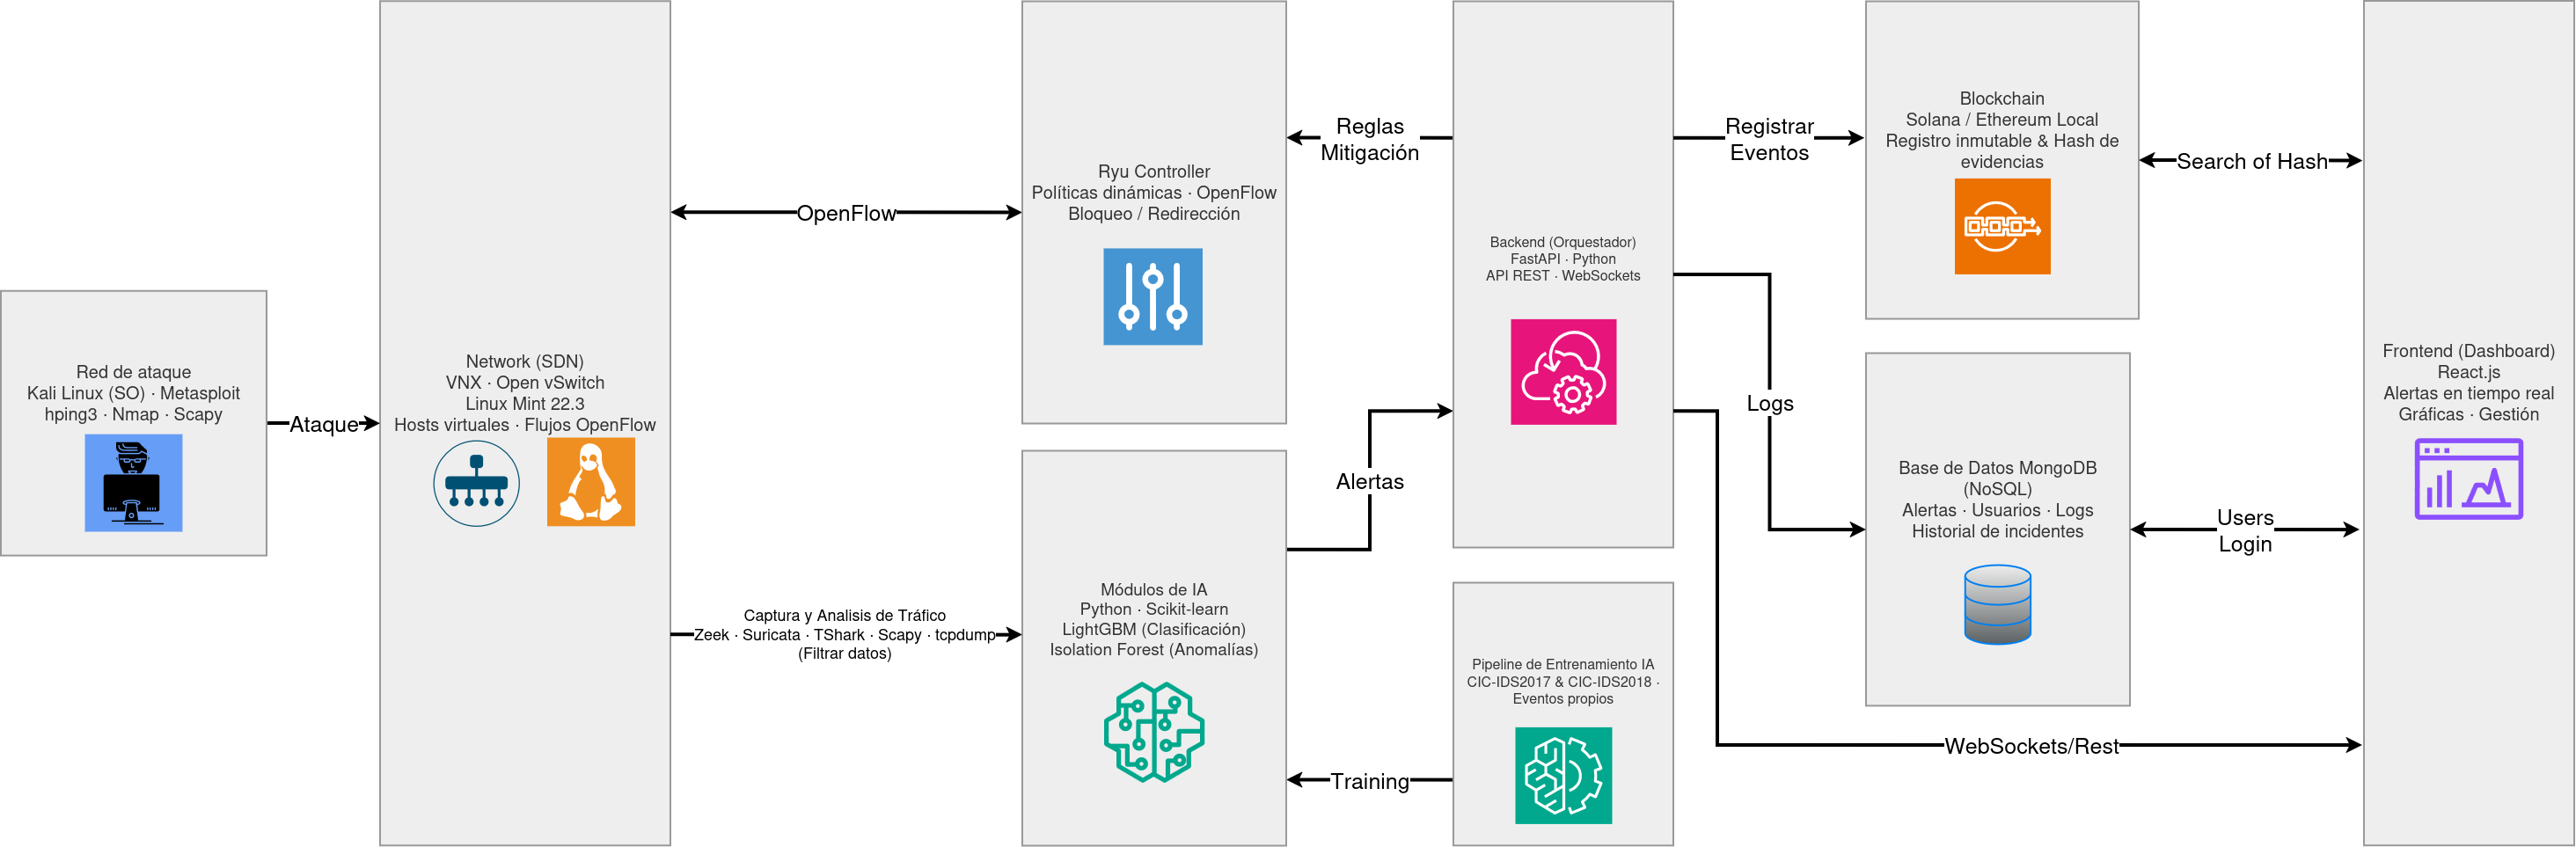
\includegraphics[width=0.95\linewidth]{recursos/cyber-defense-architecture.png}
    \caption{Arquitectura general de la plataforma de ciberseguridad propuesta.}
    \label{fig:arquitectura}
\end{figure}

\begin{description}
    \item[Capa de percepci\'on.] Captura el tr\'afico en el punto de observaci\'on de la red y lo retransmite hacia la capa de an\'alisis.
    \item[Capa de an\'alisis.] Extrae caracter\'isticas del tr\'afico, aplica el modelo de clasificaci\'on y emite los eventos de seguridad con su nivel de severidad.
    \item[Capa de control.] Traduce los eventos de seguridad en acciones de mitigaci\'on sobre el switch programable, mediante reglas de flujo din\'amicas.
    \item[Capa de presentaci\'on.] Consolida la informaci\'on en un tablero web que permite la visualizaci\'on, el an\'alisis y la gesti\'on de los incidentes.
\end{description}

La validaci\'on se realiza en un entorno virtual que reproduce la topolog\'ia del escenario del cliente: tres m\'aquinas virtuales con roles diferenciados (atacante, servidor de aplicaci\'on y servidor de datos) conectadas a un switch virtual programable, gobernado por un controlador de red. Sobre este escenario se reproducen t\'ecnicas de ataque de reconocimiento, fuerza bruta y denegaci\'on de servicio, midiendo la capacidad de detecci\'on, el tiempo de respuesta y la efectividad de la mitigaci\'on.

\section{Contribuciones}

La principal contribuci\'on del proyecto es la integraci\'on efectiva de la detecci\'on con aprendizaje autom\'atico y la mitigaci\'on sobre redes programables en una \'unica plataforma operativa, cerrando el ciclo detecci\'on--respuesta con intervenci\'n humana m\'inima. Se suman como contribuciones adicionales la validaci\'on experimental reproducible sobre un entorno virtual, la definici\'on de un modelo de despliegue aplicable a la infraestructura real del cliente y el registro auditable de los eventos de seguridad atendidos.

\section{Estructura del documento}

El presente documento se organiza en los siguientes cap\'itulos: el Cap\'itulo 1 introduce el contexto, la problem\'atica, los objetivos, el alcance y la metodolog\'ia aplicada. Los cap\'itulos siguientes desarrollan el marco te\'orico, la evaluaci\'on de riesgos y alternativas tecnol\'ogicas consideradas, los resultados experimentales obtenidos y las conclusiones y l\'ineas futuras de trabajo. Finalmente, se incluyen las referencias bibliogr\'aficas y los ap\'endices con el material complementario del proyecto.
